\chapter{Metodología}

\section{Introducción}
El prototipo del metamodelo se realizará a través de la metodología en cascada, por cronograma solo cubrirá las etapas de Análisis de Requisitos y Diseño, ya que solo se entregará un prototipo de metamodelo a la Unidad de Victimas, por lo tanto, la etapa de Implementación, Pruebas y Mantenimiento no se realizará. 
\\
En un futuro, será para toda los aplicativos de la organización, en este momento solamente se cubrirá unas
cuentas aplicaciones criticas del negocio para su centralización y trazabilidad, y se realizará en la etapa de Análisis y Diseño de acuerdo a los requerimientos de la Organización.

\section{Proceso}
El modelo en cascada es un proceso de desarrollo secuencial, en el que el desarrollo de software se concibe como  un conjunto de etapas que  se ejecutan una tras otra. Se le denomina así por las posiciones que ocupan las diferentes fases que componen el proyecto, colocadas una encima de otra, y siguiendo un flujo de ejecución de arriba hacia abajo, como una cascada.
\newpage

\begin{figure}[h!]
	\centering	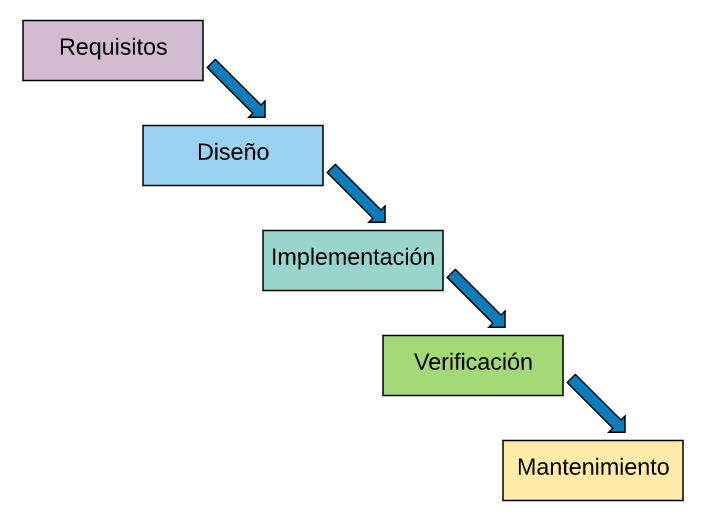
\includegraphics[width=0.5\linewidth]{Proyecto/Metodologia/imgs/MetodoCascada}
	\caption{Metodología Cascada \cite{MetSB,ID1,ID2}}
\end{figure}

El modelo de desarrollo en cascada se originó en la industria y la construcción, donde los cambios a posteriori son caros y difíciles de implementar. Cuando estás creando un producto material, realizar cambios en lo ya construido es mucho más difícil que en un programa informático. En el mundo del software, todavía no se habían implantado otras metodologías de desarrollo por lo que se adaptó el modelo en cascada que se utilizaba en otros sectores. 
\\
\\
\textbf{Fases del modelo}
\\
El modelo de desarrollo en cascada sigue una serie de etapas de forma sucesiva, la etapa siguiente empieza cuando termina la etapa anterior. Las fases que componen el modelo son las siguientes:
\\
\\
\textbf{Requisitos del software}
\\
En esta fase se hace un análisis de las necesidades del cliente para determinar las características del software a desarrollar, y se especifica todo lo que debe hacer el sistema sin entrar en detalles técnicos. Hay que ser especialmente cuidadoso en esta primera fase, ya que en este modelo no se pueden añadir nuevos requisitos en mitad del proceso de desarrollo.
\\
\\
Por lo tanto, esta es la etapa en la que se lleva a cabo una descripción de los requisitos del software, y se acuerda entre el cliente y la empresa desarrolladora lo que el producto deberá hacer. Disponer de una especificación de los requisitos permite estimar de forma rigurosa las necesidades del software antes de su diseño. Además, permite tener una base a partir de la cual estimar el coste del producto, los riesgos y los plazos.
\\
\\
En el documento en el que se especifican los requisitos, se establece una lista de los requerimientos acordados. Los desarrolladores deben comprender de forma clara el producto que van a desarrollar. Esto se consigue teniendo una lista detallada de los requisitos, y con una comunicación fluida con el cliente hasta que termine el tiempo de desarrollo.
\\
\\
\textbf{Diseño}
\\
\\
En esta etapa se describe la estructura interna del software, y las relaciones entre las entidades que lo componen.
\\
\\
Descompone y organiza el sistema en elementos que puedan elaborarse por separado, aprovechando las ventajas del desarrollo en equipo. Como resultado surge el SDD (Documento de Diseño del Software), que contiene la descripción de la estructura relacional global del sistema y la especificación de lo que debe hacer cada una de sus partes, así como la manera en que se combinan unas con otras.
\\
\\
Es conveniente distinguir entre diseño de alto nivel o arquitectónico y diseño detallado. El primero de ellos tiene como objetivo definir la estructura de la solución (una vez que la fase de análisis ha descrito el problema) identificando grandes módulos (conjuntos de funciones que van a estar asociadas) y sus relaciones. Con ello se define la arquitectura de la solución elegida. El segundo define los algoritmos empleados y la organización del código para comenzar la implementación.
\\
\\
\textbf{Implementación}
\\
\\
En esta fase se programan los requisitos especificados haciendo uso de las estructuras de datos diseñadas en la fase anterior.La programación es el proceso que lleva de la formulación de un problema de computación, a un programa que se ejecute produciendo los pasos necesarios para resolver dicho problema.
\\
\\
Al programar, tenemos que realizar actividades como el análisis de las condiciones, la creación de algoritmos,  y la implementación de éstos en un lenguaje de programación específico.
\\
\\
\textbf{Verificación}
\\
\\
Como su propio nombre indica, una vez se termina la fase de implementación se verifica que todos los componentes del sistema funcionen correctamente y cumplen con los requisitos.
\\
\\
El objetivo de las pruebas es el de obtener información de la calidad del software, y sirven para: encontrar defectos o bugs, aumentar la calidad del software, refinar el código previamente escrito sin miedo a romperlo o introducir nuevos bugs, etc.
\\
\\
\textbf{Instalación y Mantenimiento}
\\
\\
Una vez se han desarrollado todas las funcionalidades del software y se ha comprobado que funcionan correctamente, se inicia la fase de instalación y mantenimiento. Se instala la aplicación en el sistema y se comprueba que funcione correctamente en el entorno en que se va a utilizar.
\\
\\
A partir de ahora hay que asegurarse de que el software funcione y hay que destinar recursos a mantenerlo. El mantenimiento del software consiste en la modificación del producto después de haber sido entregado al cliente, ya sea para corregir errores o para mejorar el rendimiento o las características.
\\
\\
Para llevar a cabo correctamente la fase de mantenimiento, se necesita trazar un plan de antemano que nos prepare para todos los escenarios que puedan producirse durante esta fase. Para evitar futuros conflictos con el cliente, en el plan hay que especificar cómo los usuarios solicitarán las modificaciones o la corrección de errores, hacer una estimación del coste de la modificación de funcionalidades o corrección de errores, quién se encargará del mantenimiento, durante cuanto tiempo se dará soporte al software, etc.  